%!TEX root = ../Thesis.tex
\chapter{Introduction}
\justify
\noindent

\section{Copenhagen Suborbitals}

Copenhagen Suborbitals is a space organisation located in Denmark. Since 2011, they have developed and flown six internal built rockets and space capsules, launching rockets from a sailing platform in international waters (Baltic Sea). The rockets are built in a workshop in Copenhagen, Denmark. The budget is minimal compared to professional space programs, therefore the guiding principle is building  spacecraft with focus on functionality and cost-efficiency. This requires use of self-built production methods in the workshop.

The goal of the organisation is to develop technologies for flying crewed into space and return safely, which will happen with the Spica mission, which is the next phase in Copenhagen Suborbitals's space program. The previous rockets have been developed for testing technologies necessary for this mission, with considerations for human flight. The first Spica rocket will combine previous knowledge as well as new technologies, at a higher scale. 
It will be a reusable vehicle with a different thrust vector control system compared to previous rockets. It is necessary to be studied and understand the type of control systems are suitable for this rocket. 

The navigation system of this rocket will be inertial based, involving inertial measurement units with 9 degrees of freedom: accelerometer, gyroscope, magnetometer. Since the rocket is still in early stages of development, a hardware prototype simulating the rocket will be developed, which will allow to test control algorithms that will build the foundation for Spica control strategies.  

\begin{figure}[h!]
  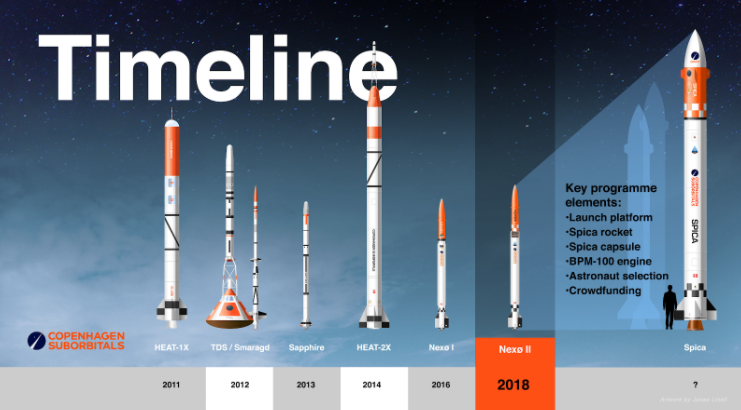
\includegraphics[scale=0.9]{graphics/timeline.png}
  \caption{Timeline of rockets launched and planned by Copenhagen Suborbitals}
  \label{timeline}
\end{figure}

\section{Motivation and Project scope}

The project has two parts: navigation and control. These parts will be investigated in regards to the challenges they experience in flight, as well investigating the workflow of building such a system.
The aim of this project is to study the control system involved in gimbaled nozzle thrust vector control and develop a workflow for control of a gimbaled engine for the duration of the powered flight, with measurements from an inertial navigation system. The rocket will have a sensor suite, however, the requirement for this project is to base the navigation of the system on an inertial measurement unit sensor only. It is also required to research options for achieving absolute heading (yaw). 

The main tasks are: understanding what is involved in rocket stability in flight and gimbaled engine TVC; building a technology demonstrator prototype simulating the rocket to test the control systems;developing a inertial state estimation system based on an inertial measurement unit; designing a controller that will use the inertial sensor data to control a system suitable for a gimbaled engine and testing the controller on a technology demonstrator prototype as a substitute for the rocket. 

Technology demonstrator was settled to be a coaxial contra rotating dual copter that simulates the thrust of a rocket and the deflection within a few degrees through a rudder, simulating the gimbal engine in one axis. Therefore, the drone will be tested in one axis (pitch axis). It is outside the scope of this project to fly the drone freely, as that would require focus on additional hardware design and building of a thrust vector control system in two axes that could sustain control in flight. It is also outside of the scope of the project to control the thrust generated by the propellers as part of the control system - as a similarity to the rocket, where the thrust is controlled by the engine control system, separated from the guidance, navigation, control. 

Another main objective of this project was interacting with hardware as part of the process, as opposed to running simulations only. This approach, although more challenging, time consuming and error-prone,  was preferred because it provides the realistic and practical view of the results, along with places to improve. Hardware implementation also allows for understanding physical limitations of the systems that most be taken intro consideration in the design and control process, such as actuator delays, slack and limits, behavior of electronic devices under different types of stress, signal processing challenges, physical misalignment issues, constraints to be taken into consideration. 

The modelling of the system was based on first principles, Newton-Euler as opposed to Lagrange - as the focus of this project is understanding the interplay of forces acting on the system. The system is modeled as a multi-body,with modeled  dynamics forces and reaction forces, along with their physical constraints. The reasoning was to allow understanding of the dynamics of the system, the separate parts acting on each other, the physical constraints and to allow mechatronic design work for the rocket based on understanding of these interactions and real-life challenges. 


\section{Requirements}

\begin{enumerate}
\item investigating sources of errors in the inertial sensor, particularly the gyro drift in flight.
\item deciding on an absolute heading (yaw) sensor to correct the gyro orientation. 
\item navigational attitude representation through a method avoiding singularities. 
\item investigating navigation filters fit for lower processing power, Arduino class micro-controllers.
\item navigation filters with a average deviation of maximum 1.5 degrees from the true value.
\item 1 axis control that can be extended to 2 or 3 axes
\item Controller with max 30 percent overshoot and 1.5 sec settling time
\end{enumerate}


\section{Comparison between hardware prototype and rocket}

The reason for using a testing platform in the form is that the rocket is not built yet, it currently at the start of its production phase and therefore, cannot be tested upon. However, the controller for such a rocket takes a long time to develop and should be developed alongside the hardware, not afterwards. Often cases, rocket attitude control systems cannot be tested on the real hardware prior to launch, therefore there is a need to be able to test on a technology demonstrator prototype instead, to assess the capabilities and performance of the controller and familiarize with hardware challenges. This is the advantage of having the drone prototype, as opposed to purely running models in simulation: it allows for testing of control algorithms and assessing the challenges that arise when working with real hardware, which simulations can only partially replicate. 

The drone and the rocket are comparable due to their similarities, which allowed for reduced scale and scope  process replication for a first iteration of the prototype. Both drone and rocket are modelled as a rigid body: drone has a rectangular frame for stability purposes when static, whereas the rocket is cylindrical for aerodynamic purposes. The navigation is based off an IMU in both bodies: the IMU of the drone is a low-cost MEMS (micro-electro-mechanical system) technology, while the IMU used in the rocket will be a high precision sensor. 
Thrust force is an important component of the thrust vector control in both bodies: in the case of the rocket, it is provided through propellant combustion, whereas the drone has air flow pushed by its two propellers. 
The drone has the advantage of being less dangerous to operate due to avoiding the combustion process and makes tests easier, safer, quicker to carry. 

\begin{figure}[H]
  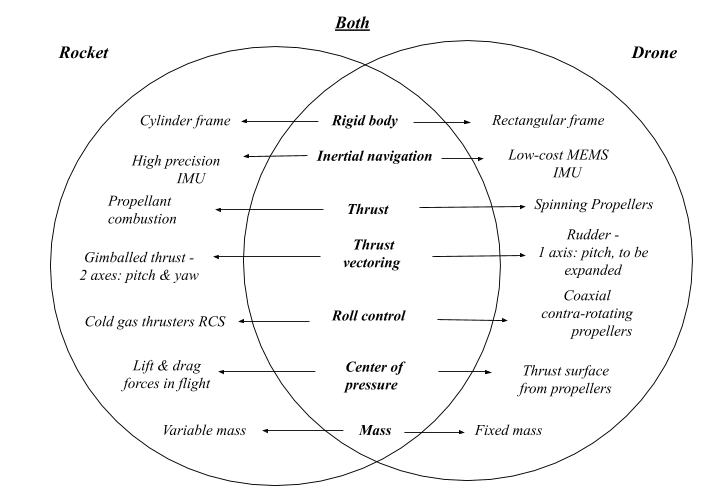
\includegraphics[scale=0.9]{graphics/Diagram.png}
  \caption{Comparison between rocket and drone}
  \label{diagramcomparison}
\end{figure}

The other component of the thrust vector control is the thrust deflection, carried in the rocket by its gimbaled engine, in two axis: pitch and yaw. 
In the case of the drone, the metal rudder handles the deflection of the propeller air flow, for now in one axis (pitch). There are three axes to both the rocket and the drone: roll, pitch and yaw. The roll axis (longitudinal) is controlled in both bodies by a separate control system. In the case of the rocket, the system is cold gas thrusters placed in the upper body of the rocket. 
The drone has roll control ensured by its two contra rotating propellers, which cancel each other’s introduced moment about the longitudinal axis. 

An important part of aerial stability is the location of the center of pressure on the rocket, relative to the center of mass. The center of pressure is the place where the aerodynamic forces act in flight. 
Although currently the drone will not be flown freely, the same principles apply for its aerial stability: it is necessary that the drone be top-heavy, like the rocket, in order to maintain the stability margin between the center of mass located above the center of pressure. 
Rocket has its center of pressure located towards bottom, near the location of its fins. The drone has its center of pressure on the area the propellers act on the rudder. The last important aspect in comparing these two systems is their mass. There is a considerable difference in their size and mass, however, they are not built to scale of each other. One of the key properties of a rocket is that the depletion of its fuel in flight leads to variable mass and moment of inertia. This is something that is not replicated by the drone at this time, drone having instead fixed mass and moment of inertia. 

\vspace{5mm}

\textbf{Similarities:}
\begin{itemize}
\item Inertial navigation
\item Drone and rocket have thrust, which allows for thrust vector control through thrust deflection 
\item Both have center of mass above the center of pressure 
\item Rocket has roll control handled by the reaction control system, drone also has roll control handled by its contra rotating propellers 
\end{itemize}


\textbf{Differences:}
\begin{itemize}
\item Rocket is combustion powered, drone’s thrust is propeller based
\item Rocket has 2 axis of control on gimbal, drone currently has 1 for its first iteration, to be expanded to 2 in future work
\item Size/scale difference 
\item Drone does not currently have variable mass to affect its moment of inertia, a common property of rockets.
\end{itemize}


\textit{Next chapter describes the rocket in more detail, as well as the considerents preceding the work on the control system. }

